\documentclass[a4paper,11pt]{jsarticle}


% 数式
\usepackage{amsmath,amsfonts}
\usepackage{bm}
% 画像
\usepackage[dvipdfmx]{graphicx}


\begin{document}

\title{カノニカル分布と自由エネルギー}
\author{須賀勇貴}
\date{最終更新日:\today}
\maketitle
長岡さんの「統計力学」を参考にした.
\vspace{0.5cm}

\section{カノニカル分布}
大きな外部の系と接触して熱平衡にある系が,いろいろなエネルギーの量子状態を取る確率分布を求める.
\subsection*{カノニカル分布}
図\ref{canonical}のように接触した2つの系A,Bがあり,BはAに比べて十分大きいとする.Aが注目する系であり,Bはその外部全体を表す.AB間にはエネルギーのやりとりがあるが,AとB全体はその外部から遮断されていて,全体のエネルギーは一定であるとする.すなわち,A,Bのエネルギーをそれぞれ$E_A,E_B$とし,全系のエネルギーを$E_T(=\text{一定})$とすれば
\begin{equation}
  E_A + E_B = E_T
\end{equation}
である.この条件の下で,$E_A,E_B$はいろいろな値をとる.\par
さて,全体が熱平衡にあるとき,Aがエネルギー$E_n$の量子状態$n$にある確率はどうなるか.Bの量子状態を$m$で示すと,全系の量子状態は$(n,m)$で表される.全系は孤立しているから,等確率の原理により,すべての量子状態$(n,m)$は等しい確率で実現すると考えられる.Aが状態$n$にあるとき,Bのエネルギーは$E_T-E_n$であり,Bはエネルギーが$E_T-E_n$の量子状態のどれかにある.したがって,Bがエネルギー$E$をもつ量子状態の数を$W_B(E)$とすれば,Aが$n$にある確率$P_n$は$W_B(E_T-E_n)$に比例する.すなわち
\begin{equation}
  P_n \propto W_B(E_T-E_n)
\end{equation}
Bのエントロピーを$S_B(E)$とすれば,
\begin{equation}
  S_B(E) = k_B \ln{W_B(E)}
\end{equation}
したがって,
\begin{equation}
  W_B(E) = \exp{\left[ \frac{1}{k_B}S_B(E) \right]}
\end{equation}
と表せるから
\begin{equation}
  P_n \propto \exp{\left[ \frac{1}{k_B}S_B(E_T-E_n) \right]}
\end{equation}
となる.\par
ここで,外部の系Bは注目する系Aに比べて十分大きいという条件を思い起こそう
を思いおこそう.エネルギーについても,$E_A \ll E_B$と考えられるから
\begin{equation}
  E_n \ll E_T
\end{equation}
としてよい.そこで,$S_B(E_T-E_n)$を$E_n$についてテイラー展開し,第2項まで残すと,
\begin{equation}
  S_B(E_T-E_n)
  \cong S_B(E_T) - \left( \frac{dS_B}{dE} \right)_{E=E_T}E_n
\end{equation}
第2項の係数は,式(\ref{})により,系Bの温度の逆数になるから,Bの温度を$T$とすれば
\begin{equation}
  P_n
  \propto \exp{\left[ \frac{1}{k_B}\left\{ S_B(E_T) - \frac{E_n}{T} \right\} \right]}
\end{equation}
ここで,$n$に依存する項のみを残し,
\begin{equation}
  P_n \propto \exp{\left[ -\frac{E_n}{k_B T} \right]}
\end{equation}
となる.確率は規格化されていなければならないから
\begin{align}
  P_n & = \frac{1}{Z}\exp{\left[ -\frac{E_n}{k_B T} \right]} \\
  Z   & = \sum_{n}\exp{\left[ -\frac{E_n}{k_B T} \right]}
\end{align}
が得られる.式(\ref{})の$n$についての和は,系Aのすべての量子状態についての和を表す.\par
温度$T$の熱平衡状態にある大きな外部の系に接して熱平衡にある,粒子数一定の系のとる式(\ref{})の確率分布をカノニカル分布(canonical distribution),または正準分布という.規格化の定数$Z$は分配関数,または状態和とよばれる.後で示すように,$Z$が決まれば,熱平衡にある系の種々の物理量をこれから求めることができる.

\subsection*{カノニカル分布が成り立つ条件}


















\begin{figure}
  \begin{center}
    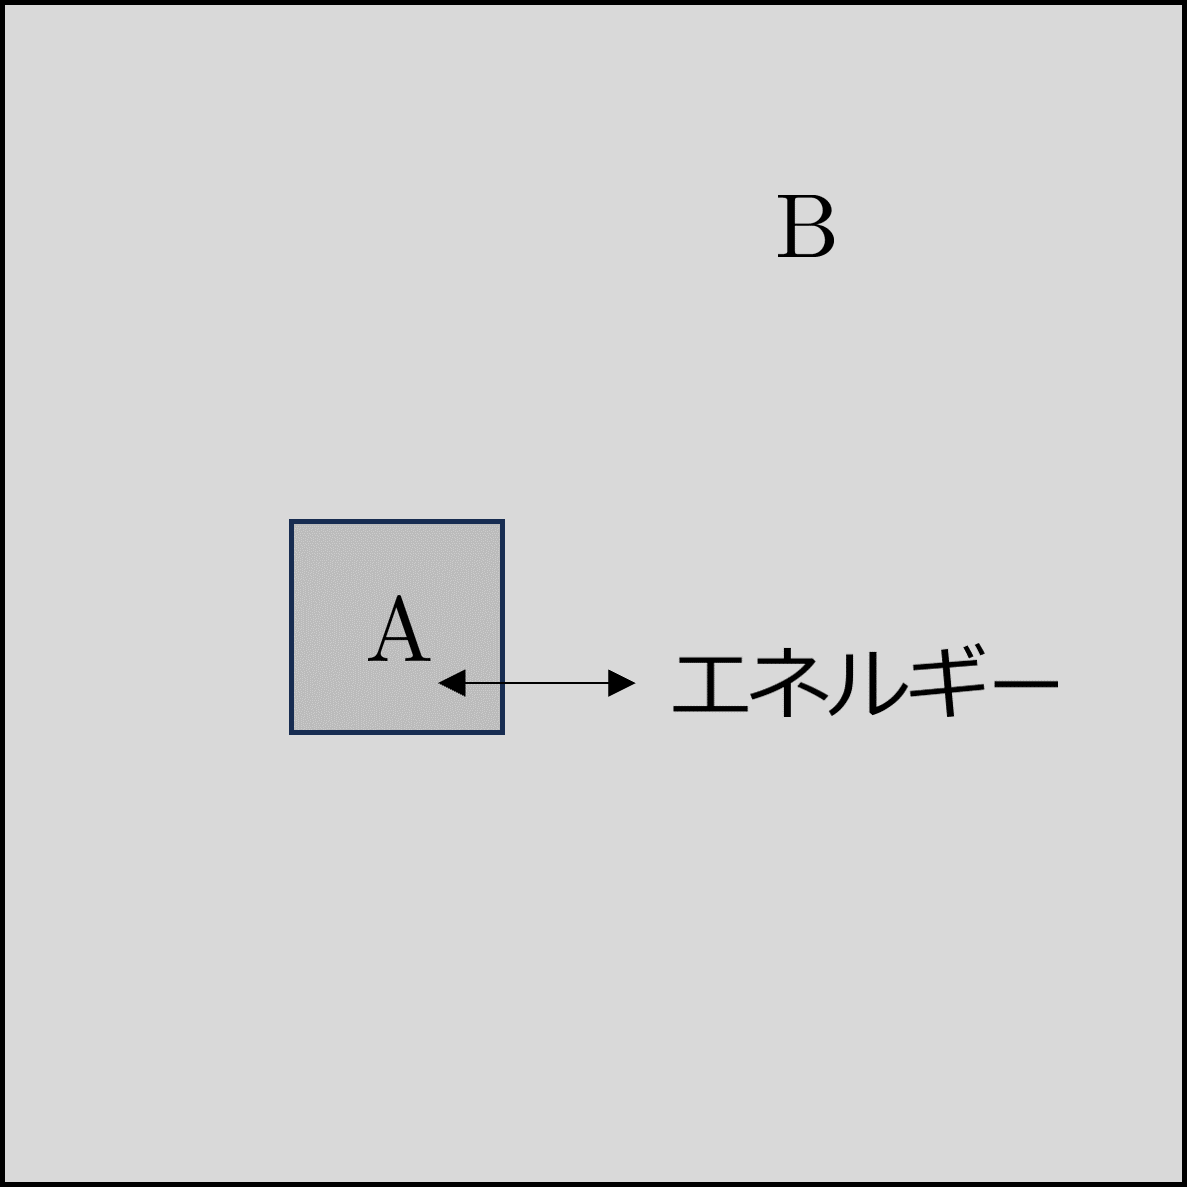
\includegraphics[height=5cm]{graph/canonical.png}
    \caption{系Aは大きな系Bと接触し,AB間にはエネルギーのやりとりが起きている\label{canonical}}
  \end{center}
\end{figure}







\end{document}